\documentclass[a4paper,10pt]{article}
\usepackage{graphicx}
\usepackage[utf8x]{inputenc}
\usepackage{times}			%
\usepackage{amssymb,amsfonts}
\usepackage[tbtags]{amsmath}
\usepackage{cite}
\usepackage{pict2e}
\usepackage{float}
\usepackage{lscape}
\usepackage[all]{xy}
\usepackage{graphics,graphicx,color,colortbl}
\usepackage{times}
\usepackage{subfigure}
\usepackage{wrapfig}
%\usepackage{multicol}
\usepackage{cite}
\usepackage{url}
\usepackage[tbtags]{amsmath}
\usepackage{amsmath,amssymb,amsfonts,amsbsy}
\usepackage{listings}
\usepackage{bm}
\usepackage{algorithm}
\usepackage{algorithmic}
\usepackage[centerlast, small]{caption}
\usepackage[colorlinks=true, citecolor=blue, linkcolor=blue, urlcolor=blue, breaklinks=true]{hyperref}
\hyphenation{ele-men-tos he-rra-mi-en-ta cons-tru-yen trans-fe-ren-ci-a pro-pu-es-tas si-mu-lar vi-sua-li-za-cion}

\usepackage{anysize}
\marginsize{2cm}{1cm}{1cm}{1cm}
\renewcommand{\abstractname}{Resumen}
\renewcommand{\figurename}{Figura}

%opening
\title{Escritura y lectura de los registros del periférico multiplicador}
\author{Oscar Andrés Urbano Vallejo}

\begin{document}

\maketitle

\begin{abstract}
 En el presente documento se explica detalladamente y a través de simulaciones, un ejemplo de escritura y lectura de los registros correspondientes al periférico multiplicador. Esto se hace con el fin de  mostrar al lector como es la interacción de las componentes software y hardware del J1. 
\end{abstract}


\begin{center}
\section*{Periférico multiplicador}
\end{center}


\begin{figure}[H]	%Diagrama de bloques del periférico multiplicador
  \centering
    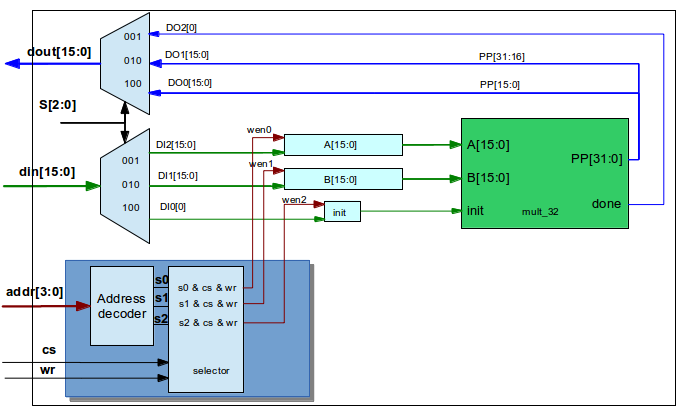
\includegraphics[scale=0.7]{diag_bloques_mult.png}
      \caption{Diagrama de bloques.}
	\label{fig1}
\end{figure}

El periférico multiplicador interactúa con el núcleo del J1  a través del siguiente mapa de memoria:

\begin{figure}[H]	%memory map multiplicador
  \centering
    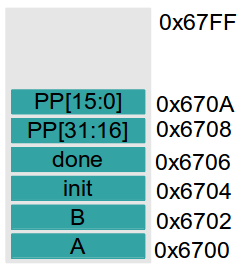
\includegraphics[scale=0.7]{memory_map_mult.png}
      \caption{Mapa de memoria.}
	\label{fig2}
\end{figure}

Los 8 bits más significativos del bus de direcciones se utilizan para habilitar la señal de Chip\_Select que para este caso (67) selecciona el periférico multiplicador. Y  a través de los 8 bits menos significativos se apunta a cada uno de los registros necesarios para operar el multiplicador.

A continuación se muestra el decodificador de direcciones (Address\_decoder, componente hardware) que se implementó para el caso del multiplicador:

\begin{figure}[H]	%addres decoder mult
  \centering
    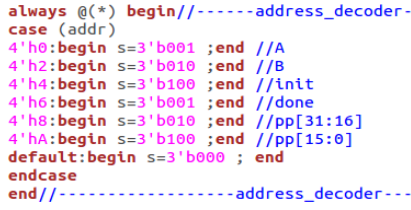
\includegraphics[scale=0.7]{addres_dec_mult.png}
      \caption{Decodificador de direcciones, verilog.}
	\label{fig3}
\end{figure}

En este caso el número de registros necesarios es inferior a 8 por lo cual con leer los 4 bits menos significativos del bus de direcciones es suficiente.

Esta sección de código lo que hace es modificar la señal s, que es la que controla el multiplexor y el demultiplexor mostrado en la figura 1, estos a su vez dirigen la información que entra por el bus de datos a su correspondiente registro. La escritura en estos registros se habilita cuando la señal de write (wr) se pone en 1.

Del lado del software es necesario hacer la definición de las direcciones que se utilizará para escribir cada registro, esto se debe hacer en el archivo hw\_defs.fs tal como se muestra en la figura 4.

\begin{figure}[H]	%mem map multiplicador
  \centering
    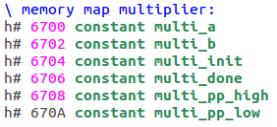
\includegraphics[scale=0.8]{mem_map_forth_mult.png}
      \caption{Definición de las direcciones de cada registro, forth.}
	\label{fig4}
\end{figure}


El código a implementar en forth debe ser escrito en el archivo app.fs.  Para este caso, haciendo uso del código mostrado en la figura 5, se interactúa con el modulo multiplicador descrito en hardware.


\begin{figure}[H]	%forth_mult
  \centering
    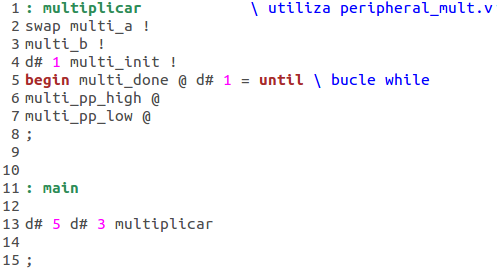
\includegraphics[scale=0.7]{forth_mult.png}
      \caption{Definición y llamado de la función multiplicar, forth.}
	\label{fig5}
\end{figure}


Primero se cargan en la pila los números 5 y 3  en formato decimal (\#d) a continuación se llama a la función multiplicar. La función multiplicar ya está previamente definida.

Esta función en la línea 2 intercambia los dos últimos valores almacenados en la pila (comando 'swap'), para de esta manera tener acceso al 5 y enviarlo al registro correspondiente a la dirección multi\_a. Posteriormente en la línea 3 el siguiente valor almacenado en la pila (en este caso el 3) es enviado a la dirección correspondiente al registro multi\_b, luego en la línea 4 el número 1 es enviado a la dirección del registro correspondiente a multi\_init, con lo que se inicia la operación del módulo multiplicador descrito en hardware.

\begin{figure}[H]	%sim_write_mult
  \centering
    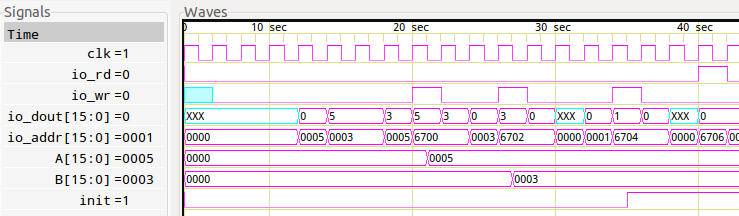
\includegraphics[scale=0.7]{sim_write_mult.png}
      \caption{Simulación escritura de registros.}
	\label{fig6}
\end{figure}

La escritura de los registros se puede observar en la simulación correspondiente a la figura 6.

En este punto el J1 ha escrito en los registros correspondientes a las direcciones multi\_a, multi\_b y multi\_init (definidos en la figura 4), el siguiente paso es esperar a que el modulo en hardware, multiplicador, envíe la señal de finalización, la cual se obtiene leyendo continuamente el registro correspondiente a la dirección multi\_done, esto es lo que hace la línea 5, (el proceso de lectura se aprecia en la figura 7) que es un bucle que no se rompe hasta que el registro multi\_done sea igual a 1.

\begin{figure}[H]	%sim_read1_mult
  \centering
    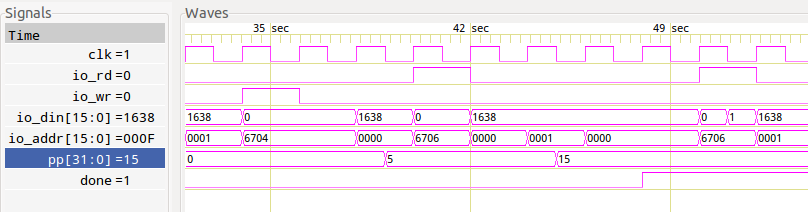
\includegraphics[scale=0.7]{sim_read1_mult.png}
      \caption{Simulación lectura de registro done.}
	\label{fig6}
\end{figure}

Una vez cumplida esta condición, es decir en el momento en que el modulo multiplicador  ya ha acabado de hacer la operación, se leen los registros correspondientes a las direcciones a las que apuntan multi\_pp\_high y multi\_pp\_low que es donde queda almacenado el resultado de la multiplicación (figura 8).

\begin{figure}[H]	%sim_read2_mult
  \centering
    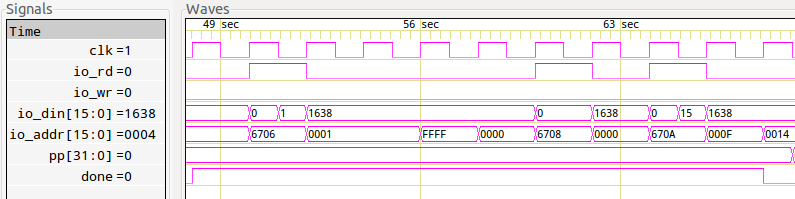
\includegraphics[scale=0.7]{sim_read2_mult.png}
      \caption{Simulación lectura registros pp.}
	\label{fig7}
\end{figure}

Y con esto el resultado de la multiplicación ya se tienen almacenado en las direcciones correspondientes a multi\_pp\_high y multi\_pp\_low.

Esta es la forma en que el J1 utiliza un programa definido en forth e interactúa con los periféricos descritos en hardware. Entender esta unión o proceso de comunicación entre ambas partes es de vital importancia, ya que con estos conceptos claros, se pueden agregar los módulos que se desee al J1 y adecuarlo así a las necesidades del proyecto.


\end{document}

